\section{Obálka sfér}
Označme $X \in \mathbb{R}^3$ a predpokladajme, že $m(t) \colon I \subset \mathbb{R} \rightarrow \mathbb{R}^3$ je parametrizácia krivky $m$ a $r(t) \colon I \rightarrow \mathbb{R}^{+}$ je funkcia definovaná na tom istom intervale. Krivka $m$ sa nazýva kostrová krivka obálky (\textit{spine curve}) a $r$ sa nazýva funkcia polomeru (\textit{radius function}). Jednoparametrický systém sfér $\mathcal{S}$ je daný rovnicou

$$
F(X, t) = \langle X - m(t), X - m(t) \rangle - r^2(t)= 0.
$$

Podľa definície \ref{charakterizacia}, obálku $\mathcal{E}$ možno nájsť ako prienik systému sfér $\mathcal{S}$ a ich derivácií $\mathcal{\dot{S}}_t$ pre všetky $t \in I$. Derivácia $\mathcal{S}$ nám dáva roviny $\mathcal{\dot{S}}$ dané rovnicou

$$
\dfrac{\partial F}{\partial t} (X, t) = \langle \dot{m}(t), X - m(t) \rangle + r(t) \dot{r}(t) = 0.
$$
Pre nájdenie obálky $\mathcal{E}$ budeme teda hľadať prieniky sféry $\mathcal{S}_t$ a roviny $\mathcal{\dot{S}}_t $ pre každý parameter $t \in I$.

\subsection{Charakteristická kružnica}
\begin{definition}[Charakteristická kružnica]
V prípade, že pre $t \in I$ je $\mathcal{S}_{t} \cap \mathcal{\dot{S}}_{t} \neq \emptyset$, sa tento prienik nazýva sa charakteristická kružnica $c_{t}$. V prípade $\mathcal{S}_{t} \cap \mathcal{\dot{S}}_{t} = \emptyset$, pre \(t\) neexistuje žiadna charakteristická kružnica.
\end{definition}

\begin{lemma} \label{lema o zjednoteni charakteristickych kruznic}
Zjednotenie všetkých charakteristických kružníc $c_{t}$ jednoparametrického systému sfér $\mathcal{S}_t$ je obálka $\mathcal{E}$ tohto systému, teda platí $$\mathcal{E} = \bigcup_{t \in I} c_{t}.$$
\end{lemma}

\begin{proof}
Nech bod $X$ patrí do zjednotenia kružníc $ \bigcup_{t \in I} c_{t}, $ potom existuje aspoň jedno $t_0 \in I, $ pre ktoré $X \in c_{t_0}.$ Keďže $c_{t_0} = \mathcal{S}_{t_0} \cap \mathcal{\dot{S}}_{t_0}, $ tak sú rovnice $\mathcal{S}_{t_0} $ a $ \mathcal{\dot{S}}_{t_0}$ splnené pre nejaké $t_0$ a $X,$ a preto patrí $X$ obálke $\mathcal{E}, $ a teda platí inklúzia $\bigcup_{t \in I} c_{t} \subseteq \mathcal{E}. $

Opačne, ak $X$ patrí obálke $\mathcal{E},$ existuje podľa definície \ref{charakterizacia} $t_0 \in I $ také, že platí $F(X,t_0) = 0$ a súčasne $\dfrac{\partial F}{\partial t}(X, t_0)=0,$ to znamená, že $X$ leží v prieniku $\mathcal{S}_{t_0} \cap \mathcal{\dot{S}}_{t_0} = c_{t_0} $ a $c_{t_0} \subseteq \bigcup_{t \in I} c_t. $ Preto platí inklúzia $\mathcal{E} \subseteq \bigcup_{t \in I} c_t.$ 

Týmto je rovnosť $\mathcal{E} = \bigcup_{t \in I} c_t$ dokázaná.
\end{proof}

Obálka sfér sa teda skladá zo systému kružníc. Charakteristická kružnica leží celá v rovine $\mathcal{\dot{S}}_t $, takže v tejto rovine leží aj jej stred. Dotykový vektor kostrovej krivky $m(t)$ je kolmý na rovinu $\mathcal{\dot{S}}_t$, teda stred $C_t$ charakteristickej kružnice leží na dotyčnici $T(t, s)= m(t) + s \cdot \dot{m}(t),$ $s \in \mathbb{R}$, preto stred $C_t$ nájdeme ako
$$ \mathcal{\dot{S}}_t \cap T(t, s).$$
Pre parameter $s$ potom platí $s = \dfrac{r(t) \dot{r}(t)}{\langle \dot{m}(t), \dot{m}(t) \rangle }, $
po dosadení do $T(t, s)$ získavame
\begin{equation}
\label{eq:stred charakteristickej kruznice}
C_t = m(t) - \frac{r(t) \dot{r}(t)}{\langle \dot{m}(t), \dot{m}(t) \rangle} \dot{m}(t).
\end{equation}

Rozoberme si nasledujúce dva prípady
\begin{itemize}
\item Ak je funkcia polomeru $r(t)$ konštantná, $\dot{r} \equiv 0$ a rovina $\mathcal{\dot{S}}_t$ obsahuje stred sféry $M_t$ pre všetky $t \in I$, v tomto prípade možno obálku $\mathcal{E}$ považovať za posunutie (\textit{offset}) kostrovej krivky $m$. Tieto obálky sú známe ako rúrkové plochy (\textit{pipe surfaces}). Keďže rovina $\mathcal{\dot{S}}_t$ charakteristickej kružnice $c_t$ obsahuje stred sféry $M_t$ v každom $t \in I$, charakteristická krivka je hlavnou kružnicou sféry a obálka $\mathcal{E}$ je pokrytá jednoparametrickým systémom zhodných kružníc.
\item Ak funkcia polomeru $r(t)$ nie je konštantná, potom $\dot{r}(t) \neq 0$ a rovina $\mathcal{\dot{S}}_t$  neprechádza stredom sféry $M_t$. V tomto prípade obálka $\mathcal{E}$ patrí do triedy kanálových plôch.
\end{itemize}

Polomer $l_t$ charakteristiskej kružnice  možno vypočítať z pravouhlého trojuholníka $M_tC_tP,$ kde $P$ je ľubovoľný bod na charakteristickej kružnici $c_t$, a teda aj na sfére $\mathcal{S}_t.$
$$ l_t = \sqrt{r^2(t) - \|M_tC_t\|^2} = r(t) \sqrt{ 1 - \frac{\dot{r}^2(t)}{\langle \dot{m}(t), \dot{m}(t) \rangle}}. $$
V prípade, že $ \|M_tC_t\| > r(t)$, sféra $\mathcal{S}_t$ nemá s obálkou $\mathcal{E}$ reálny kontakt. 

\begin{example}
Uvažujme kostrovú krivku $m(t)$ a polomer $r(t)$
$$ 
m(t) = \begin{pmatrix} 0 \\ 0 \\ t \end{pmatrix} \quad \text{ a } \quad r(t) = \frac{t}{\sqrt{26}}.
$$
potom obálka systému je daná rovnicami
\begin{align*}
&\mathcal{S}_t \colon x^2 + y^2 + (z - t)^2 - \frac{t^2}{26} = 0, \\
&\mathcal{\dot{S}}_t \colon z - \frac{25}{26}t = 0. \\
\end{align*}
Počítajme $ \mathcal{S}_t \cap \mathcal{\dot{S}}_t $ pre všetky $t \in \mathbb{R}.$ Z druhej rovnice dostaneme $t = \frac{26}{25}z$. Po dosadení do prvej rovnice, dostávame implicitnú rovnicu pre obálku $\mathcal{E}$
$$
x^2 + y^2 - \frac{1}{25}z^2 = 0,
$$
čo je rovnica rotačného kužeľa.

Napríklad, pre $t = 1 \in I$ charakteristická krivka je prienikom dvoch plôch daných
\begin{align*}
&\mathcal{S}_1 \colon x^2 + y^2 + (z - 1)^2 - \frac{1}{26} = 0, \\
&\mathcal{\dot{S}}_1 \colon z - \frac{25}{26} = 0. \\
\end{align*}
Z toho môžeme usúdiť, že charakteristická krivka $c_1$ je kružnica so stredom v bode $C_1 = (0, 0, \frac{25}{26})$ v rovine $z = \frac{25}{26}$ a neprechádza stredom sféry $M_1 = m(1) = (0,0,1)$, polomer $c_1$ je $l_{1} = \frac{\sqrt{25}}{26}$. Vzdialenosť bodov $ \|M_tC_t\| = \frac{1}{26}$ a $r(1)= \frac{1}{\sqrt{26}}$, takže platí, že $r(1) > \|M_tC_t\|$ a sféra $\mathcal{S}_1$ má s obálkou $\mathcal{E}$ reálny kontakt.
\end{example}

Jedným z dôležitých výsledkov je, že kanálové plochy, definované ako obálka jednoparametrického systému sfér s racionálnou funkciou polomeru $r(t)$ a stredmi v racionálnej krivke $m(t)$ možno racionálne parametrizovať. \cite{Pet97}

Bohužiaľ, vo väčšine prípadov sú rovnice, ktoré charakterizujú obálky, príliš zložité a odvodiť z nich rovnicu obálky nie sme schopní.

Rúrkové povrchy sa často objavujú pri výrobe potrubia. Hladké spojenie medzi dvoma nie nevyhnutne valcovými rúrami $\mathcal{P}_1$ a $\mathcal{P}_2$ sa modeluje tak, aby bol prechod hladký, bez záhybov, vodotesný alebo dokonca aj parotesný. Na to sa používa technika \textit{rolling ball blends}, využívajúca nasledujúcu myšlienku: Kým sa sféra $S$ s konštantným alebo nekonštantným polomerom $r$ kotúľa na oboch rúrach súčasne, zanecháva stopu $s_i$ na oboch rúrach. Zmiešavacia plocha je tá časť obálky $\mathcal{E}$ jednoparametrického systému sfér, ktorá leží medzi dvoma stopami $s_1$ a $s_2$. Kostrová krivka obálky $\mathcal{E}$ je priesečníkom ekvidištánt \textit{(offsetov)} plôch $\mathcal{P}_1$ a $\mathcal{P}_2$ vo vzdialenosti $r$. Každá charakteristická krivka spája dva dotykové body zmiešavacej plochy a plochami $\mathcal{P}_1$ a $\mathcal{P}_2$, ktoré sa majú zmiešavať. Viac detailov možno nájsť v \cite{Kar00} a \cite{Ode20}. Na obrázku \ref{fig:rolling_ball_blends} vľavo je znázornená metóda so sférou s konštantným polomerom $r$, vpravo s nekonštantným.

\begin{figure}[H]
	\centering
	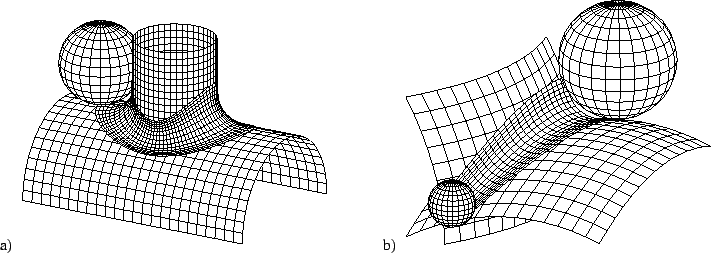
\includegraphics[width=\textwidth]{images/rolling_ball_blends.png}
	\caption[Technika rolling ball blends.]{Technika rolling ball blend s konštatným polomerom vľavo, s nekonštantným polomerom vpravo. \cite{Rollingballblends}}
	\label{fig:rolling_ball_blends}
\end{figure}

\subsection{Lokálny prienik}
V časti \ref{lokalne prieniky pre krivky} sme odvodili vzťahy medzi lokálnym prienikom jednoparametrického systému a jeho obálkou. Pre systém kružníc však platí viac ako inklúzia jedným smerom.

\begin{lemma} \label{lema o lokalnom prieniku sfer}
Lokálny prienik $\mathcal{L}_{t}$ jednoparametrického systému sfér $\mathcal{S}$ pre $t \in I$ zodpovedá charakteristickej kružnici $c_{t}$. Platí $$
\mathcal{L}_{t} = c_{t}.
$$
\end{lemma}

\begin{proof}
Ukážeme, že lokálny prienik dvoch nekonečne blízkych sfér $\mathcal{S}_{t_1}$ a $\mathcal{S}_{t_2}$ pre $\varepsilon = t_2 - t_1$ idúce k nule, bude práve charakteristická kružnica $c_{t_2}$ a to tak, že pomocou orientovanej vzdialenosti stredov sfér ukážeme, že stred charakteristickej kružnice a stred prieniku dvoch sfér sú rovnaké.
Označme ľubovoľný bod $S \in \mathcal{S}_{t_1} \cap \mathcal{S}_{t_2}$ a $M_1 = m(t_1) $ a $M_2 = m(t_2).$ Ďalej označme $l$ vzdialenosť medzi bodmi $S$ a $C,$ kde $C$ je bod ležiaci na priamke $M_1M_2$ a zároveň stred priesečníkovej kružnice. $\vec{t} $ bude jednotkový vektor v smere $ M_2 - M_1.$
Označme ako $d_1$ orientovanú vzdialenosť $M_1$ a $C$ a podobne $d_2$ orientovanú vzdialenosť $M_2$ a $C.$
$$ d_1 = \langle \vec{t}, C - m(t_1) \rangle \quad \text{a} \quad d_2 = \langle m(t_2) - C,  \vec{t} \rangle, $$
kde $d_1 + d_2 = | M_2 - M_1 |.$

 Keďže $M_1CS$ a $M_2CS$ sú pravouhlé, môžeme vyjadriť dĺžku spoločnej odvesny $l.$
$$l^2 = r^2(t_1) - d^2_1 = r^2(t_2) - d^2_2,$$
kde $d_2 = |m(t_2) - m(t_1)| - d_1, $
potom možno $d_1$ vyjadriť ako 
$$d_1 = \dfrac{ | m(t_2) - m(t_1) |}{2} - \dfrac{\dfrac{r(t_2)-r(t_1)}{t_2-t_1} (r(t_2) +r(t_1))}{\dfrac{ | m(t_2)-m(t_1) |}{t_2 - t_1}}.$$
Pre $\varepsilon = t_2 - t_1 $ idúce k nule
$$ d_1 = - \dfrac{\dot{r}(t_1) r(t_1)}{| \dot{m}(t_1) |}.  $$
Odkiaľ stred priesečníkovej kružnice je
$$S = m(t) + d_t \dfrac{\dot{m}(t)}{| \dot{m}(t)|} = m(t) - \dot{m}(t)\dfrac{r(t)\dot{r}(t)}{|\dot{m}(t)|}. $$
Tento stred $S$ zodpovedá rovnici \ref{eq:stred charakteristickej kruznice} pre stred $C_t$ charakteristickej kružnice $c_t$. Nekonečne blízke sféry sa pretínajú pre $t$ v rovine $\mathcal{\dot{S}}_{t}$, a preto je prienik daný ako 
$$ \mathcal{L}_{t} = \mathcal{S}_{t} \cap \mathcal{\dot{S}}_{t} = c_{t}. $$
V prípade, že lokálny prienik $\mathcal{L}_{s}$ pre nejaké $s \in I$ prázdny, neexistuje pre $s$ žiadna charakteristická kružnica a uvedená rovnosť stále platí.
\end{proof}

\begin{theorem}
Obálka $\mathcal{E}$ jednoparametrického systému sfér $\mathcal{S}$ pozostáva z bodov prieniku infinitezimálne blízkych prvkov systému a platí $$
\mathcal{L} = \mathcal{E}.
$$
\end{theorem}

\begin{proof}
Z predchádzajúcich dvoch lem, lemy \ref{lema o zjednoteni charakteristickych kruznic} a \ref{lema o lokalnom prieniku sfer} platí 
$$ \mathcal{E} = \bigcup_{t \in I } c_t = \bigcup_{t \in I} \mathcal{L}_t = \mathcal{L}. $$
\end{proof}

\subsection{Lokálny samoprienik}
Lokálny samoprienik obálky jednoparametrického systému guľových plôch je špeciálnym typom samopretínania obálky. Je definovaný nasledovne.
\begin{definition} \label{definicia lokalny samoprienik}
Lokálny samoprienik $\mathcal{L}_{t}$ pre $t$ je priesečníkom infinitezimálne blízkych charakteristických kružníc $c_{t}$ systému $\mathcal{S}$. Lokálny samoprienik obálky $\mathcal{E}$ je množina všetkých takých samoprienikov pre všetky parametre systému $\mathcal{S}$. Označíme ho ako $$\mathcal{L} = \bigcup_{t \in I} \mathcal{L}_t.$$
\end{definition}

Nasledujúci výrok predstavuje dôležité kritérium na identifikáciu lokálneho samoprieniku.
\begin{lemma} \label{kriterium o lokalnom samoprieniku}
Bod $Q \in \mathbb{R}^3$ patrí práve vtedy do lokálneho samoprieniku $\mathcal{L}_{t}$ obálky $\mathcal{E}$, ak sú splnené rovnice
\begin{align*}
F(Q,t) &= 0, \\
\dfrac{\partial F}{\partial t}(Q,t) &= 0, \\
\dfrac{\partial^2 F}{\partial t^2}(Q,t) &= 0
\end{align*}
pre nejaké $t \in I.$
\end{lemma}

\begin{proof}
Ľubovoľný bod $Q \in \mathcal{L}_{t}$ patrí podľa definície k priesečníku infinitezimálne blízkych kruhov pre $t$. V bode $Q$ sa navzájom pretínajú aj roviny $\mathcal{\dot{S}}_t$, v ktorých sa tieto kružnice nachádzajú. Tieto roviny patria do systému $\mathcal{\dot{S}}$, ktorý je definovaný ako množina bodov spĺňajúcu funkciu $\dfrac{\partial F}{\partial t}(Q, t)$, a sú tiež infinitezimálne blízko, to znamená, že platí $\dfrac{\partial^2 F}{\partial t^2}(Q,t) = 0, $ teda
\begin{equation}
\label{eq:druha derivacia}
\langle \ddot{m}(t), Q-m(t) \rangle - \langle \dot{m}(t), \dot{m}(t) \rangle + \dot{r}^2(t) + r(t)\ddot{r}(t) = 0. 
\end{equation}
Bod $Q$ leží na charakteristickej kružnici $c_{t},$ preto spĺňa rovnice $F (Q, t)$ a $\dfrac{\partial F}{\partial t}(Q, t).$
Opačne, predpokladajme, že sú všetky rovnosti z tejto lemy splnené pre nejaké $t \in I$ a $Q \in \mathbb{R}^3, $ potom platí
\begin{align*}
Q &\in \lim_{\varepsilon \to 0} \left( \mathcal{S}_t \cap \mathcal{S}_{t + \varepsilon} \cap \mathcal{\dot{S}}_t \cap \mathcal{\dot{S}}_{t + \varepsilon} \right) \\
&= \lim_{\varepsilon \to 0} \left( \underbrace{\mathcal{S}_t \cap \mathcal{\dot{S}}_t}_{c_{t}} \cap \underbrace{\mathcal{S}_{t + \varepsilon} \cap \mathcal{\dot{S}}_{t + \varepsilon}}_{c_{t + \varepsilon}} \right) 
\\
&= \lim_{\varepsilon \to 0} \left( {c_{t}} \cap {c_{t+ \varepsilon}} \right) \\
&= \mathcal{L}_{t}.
\end{align*}
Týmto sme ukázali, že bod $Q$ patrí do samoprieniku charakteristických kružníc pre $t$ a podľa definície \ref{definicia lokalny samoprienik} patrí do lokálneho samoprieniku $\mathcal{L}_{t}$ obálky $\mathcal{E}$.
\end{proof}

Pomocou lemy \ref{kriterium o lokalnom samoprieniku} možno ľahko rozhodnúť, či bod $Q \in \mathbb{R}^3$ pre parameter $t_0 \in I$ patrí do lokálneho samoprieniku $\mathcal{L}_{t_0}.$ Ak je $t_0$ neznáme, mohli by sme určiť $t_i$ ako riešenia rovnice $\dfrac{\partial^2 F}{\partial t^2}(Q, t_i)$. Ak by pár $(Q, t_i)$ spĺňal obe ďalšie rovnice $F(Q, t_i)$ a $ \dfrac{\partial F}{\partial t}(Q, t_i)$, bod $Q$ patrí do lokálneho samoprieniku obálky $\mathcal{E}$ pre $t_i.$

Často však riešime otázku, či obálka má lokálny samoprienik a ak áno, pre aké hodnoty parametrov $t \in I$. Pre túto otázku nie je použitie lemy \ref{kriterium o lokalnom samoprieniku} vhodné, preto predkladáme lepšie kritérium. Pozrieme sa na to z geometrického hľadiska. Rovnica \ref{eq:druha derivacia} definuje systém rovín $\mathcal{\ddot{S}}$. Pre každé $t \in I$ je vektor $\ddot{c}(t)$ kolmý na $\mathcal{\ddot{S}}_t.$ Prvé dve rovnice z lemy \ref{eq:druha derivacia} definujú pre pevné $q \in I$ charakteristickú kružnicu $c_q$, to znamená, že pre $q$ existuje lokálny samoprienik $\mathcal{L}_q$, ak sa $c_q$ a $\mathcal{\ddot{S}}_q$ pretínajú. 

Keďže roviny $\mathcal{\dot{S}}_q $ aj $\mathcal{\ddot{S}}_q $ sú rovnobežné s vektorom $ \dot{\vec{m}}(q) \times \ddot{\vec{m}}(q) $, môžu byť obe roviny projektované do roviny obsahujúcej $ m(q) $ a kolmej na $ \vec{b}_q $ a problém priesečníka môžeme takto vyriešiť v projekcii. Pod $ \vec{b}_q $ sa rozumie binormálový vektor definovaný v bode krivky $ m(q) $. Nech $\vec{n}_q$ je zodpovedajúci normálový vektor. Označme prienik priamok $C_q + s \cdot \vec{n}_q$, $s \in \mathbb{R}$, s rovinou $\mathcal{\ddot{S}}_t$ ako $S_t = C_q + s_t \cdot \vec{n}_q$ s prislúchajúcim parametrom $s_t \in \mathbb{R}$. Bod $S_t$ lokálneho prieniku pre $q$ existuje, ak jeho vzdialenosť od stredu $C_t$ charakteristickej kružnice $c_t$ je menšia ako jej polomer $l_t.$ 

\begin{align*}
| S_t - C_t | &= | s_t \cdot \vec{n}_t | = | s_t | \leq l_t.
\end{align*}

Toto je ďalšie kritérium pre existenciu lokálneho prieniku. Na určenie parametra priesečníka $ s_t $ sa pozrieme na nasledovnú rovnicu. Do rovnice \ref{eq:druha derivacia} dosadíme vyjadrenie pre bod prieniku.

\begin{align*}
\langle \ddot{m}(t), C_t + s_t \cdot \vec{n}(t) - m(t) \rangle - \langle \dot{m}(t), \dot{m}(t) \rangle + \dot{r}^2(t) + r(t)\ddot{r}(t) = 0
\end{align*}

Odkiaľ pre parameter $ s_t $ dostávame vyjadrenie

\begin{align*}
s_t &= \dfrac{ r(t) \dot{r}(t) \langle \dot{m}(t), \ddot{m}(t) \rangle + \langle \dot{m}(t), \dot{m}(t) \rangle^2 - \left( \dot{r}^2(t) + r(t)\ddot{r}(t) \right) \langle \dot{m}(t), \dot{m}(t) \rangle}{\langle \dot{m}(t), \dot{m}(t) \rangle \langle \ddot{m}(t) , \vec{n}(t) \rangle}.
\end{align*}

Tento výraz je síce dosť zložitý, avšak umožňuje identifikovať intervaly parametra $ t $, v ktorých existuje lokálny priesečník obálky $ \mathcal{E} $ prostredníctvom nájdenia koreňov funkcie $ g(t) = | s_t | - l_t $. Samotné priesečníky pre to však nemusia byť známe.

\textit{Pozorovanie:}
Pomocou kritéria je samozrejme možné efektívne rozhodnúť o tom, či sa obalová plocha lokálne pretína v určitom parametri $t \in I$ bez toho, aby sme poznali priesečníky bodov. Tie sa potom dajú ľahko určiť pomocou
$$
S_{\pm} = C_{t} + s_{t} \cdot \vec{n}_{t} + b_{\pm} \cdot \vec{b}_{t},
$$
kde $ b_{-} \in \mathbb{R} $ a $ b_{+} \in \mathbb{R} $ a $s_t^2 + b_{\pm}^2 = l_t^2 $ z pravouhlých trojuholníkov $C_{t}S_{-}S_{t}$ a $C_{t}S_{+}S_{t}.$

\subsection{Konštantný polomer}
V prípade, že je funkcia polomeru $r(t) \equiv r $ konštantná, platí $C_t = M_t,  l_t = r$ a $\dot{r} = 0,$ preto 
$$\dfrac{\partial^2 F}{\partial t^2} = s_t \cdot \langle \ddot{m}(t), n(t) \rangle - \langle \dot{m}(t), \dot{m}(t) \rangle = 0$$
a kritérium pre existenciu lokálneho prieniku $\mathcal{L}_t$ sa zjednoduší na
$$
\lvert s_t \rvert = \frac{\langle \dot{m}(t), \dot{m}(t) \rangle}{\langle \ddot{m}(t), n(t) \rangle} \leq r.
$$
\begin{example}
Pre prípad, že stredová krivka je daná normálnou parabolou, platí pre jej parametrizáciu a derivácie

\[
m(t) = \begin{pmatrix} t \\ t^2 \\ 0 \end{pmatrix}, \quad \dot{m}(t) = \begin{pmatrix} 1 \\ 2t \\ 0 \end{pmatrix} \quad \text{a} \quad \ddot{m}(t) = \begin{pmatrix} 0 \\ 2 \\ 0 \end{pmatrix}.
\]
Z toho ľahko získame vektory 
$$ \dot{m}(t) \times \ddot{m}(t) =
\begin{pmatrix} 0 \\ 0 \\ 2 \end{pmatrix} , \quad \vec{b}(t) = \begin{pmatrix} 0 \\ 0 \\ 1 \end{pmatrix} \quad  \text{a} \quad \vec{n}(t) = \dfrac{1}{\sqrt{4t^2 + 1}} \begin{pmatrix} -2t \\ 1 \\ 0 \end{pmatrix}.$$
Ak je polomer konštantný, dostávame pre parameter samoprieseku
$$ s_t = \dfrac{\sqrt{4t^2 + 1}^3}{2}, $$
ktorý je rovný obrátenej hodnote krivosti krivky $m(t)$ a to
$$ \kappa(t) = \frac{\lVert  \dot{m}(t) \times \ddot{m}(t) \rVert}{\lVert \dot{m}(t) \rVert^3} = \frac{2}{\sqrt{4t^2 + 1}^3}. $$
Zrejme platí, že $s_t$ je vždy väčšie alebo rovné $\frac{1}{2}$. To znamená, že pre všetky polomery $r < \frac{1}{2}$ neexistuje žiadny lokálny prienik. Väčšie polomery vedú k lokálnemu pretínaniu obálky pre hodnoty parametrov $t$ v intervale $[-a, a],$ kde $a \in \mathbb{R}^+ \setminus {0}$. Napríklad pre $r = 1$ platí $a = \frac{1}{2} \sqrt{2 \sqrt{3} - 1} \approx 0.38$.
\end{example}

Vzťah medzi krivosťou a parametrom priesečníka neplatí len pre tento konkrétny príklad, ale vo všeobecnosti.

\begin{lemma}
Pre obálku $\mathcal{E}$ jednoparametrického systému sfér $\mathcal{S}$ s konštantným polomerom $r(t) \equiv r \in \mathbb{R}$ je splnená rovnosť 
$$ s_t = \dfrac{1}{\kappa(t)} $$
pre všetky $t \in I$, kde $\kappa$ je krivosť kostrovej krivky $m(t).$
\end{lemma}

\begin{proof}
Označme $\alpha_t $ uhol medzi $m(t)$ a $\dot{m}(t)$ a $\beta_t $ uhol medzi $n(t)$ a $\ddot{m}(t)$. Potom platí $\alpha_t = 90 - \beta_t$ alebo $\alpha_t = 90 + \beta_t$. V oboch prípadoch je $\sin (\alpha_t) = \cos (\beta_t).$ Počítajme veľkosť parametra $s.$
\begin{align*}
|s_t| &= \dfrac{| \langle \dot{m}(t), \dot{m}(t) \rangle |}{ |\langle \ddot{m}(t), n(t) \rangle |} = \dfrac{| \dot{m}(t) |^2}{| \ddot{m}(t) | | n(t) | \cos \beta_t } = \dfrac{| \dot{m}(t) |^3}{| \dot{m}(t) | | \ddot{m}(t) | \sin \alpha_t } = \dfrac{| \dot{m}(t) |^3}{ | \dot{m}(t) \times \ddot{m}(t) | } \\
&= \dfrac{1}{\kappa (t)}
\end{align*} 
\end{proof}